
\documentclass[10pt,a4paper]{article}
\usepackage[a4paper,margin=14mm,top=18mm,bottom=20mm,headheight=12pt,headsep=5mm,footskip=9mm]{geometry}
\usepackage{fontspec}
\usepackage{xcolor}
\usepackage{graphicx}
\usepackage{tikz}
\usepackage{tabularx}
\usepackage{array}
\usepackage{fancyhdr}
\usepackage{needspace}
\usepackage{multicol}
\usepackage{enumitem}
\defaultfontfeatures{Ligatures=NoCommon}
\IfFontExistsTF{Noto Sans CJK SC}{\setmainfont{Noto Sans CJK SC}\setsansfont{Noto Sans CJK SC}}{\setmainfont{DejaVu Sans}\setsansfont{DejaVu Sans}}
\IfFontExistsTF{DejaVu Sans}{\newfontfamily\BOQuoteFont{DejaVu Sans}}{\newfontfamily\BOQuoteFont{Latin Modern Sans}}
\newcommand{\BOApos}{{\BOQuoteFont\char"0027}}
\definecolor{BOBlue}{HTML}{0E6B72}
\definecolor{BOBright}{HTML}{20A66A}
\definecolor{BOGreen}{HTML}{00A651}
\definecolor{BONavy}{HTML}{1B2A34}
\definecolor{BOText}{HTML}{24323A}
\definecolor{BOMuted}{HTML}{7C878E}
\definecolor{BOLine}{HTML}{D9E1E6}
\definecolor{BOLight}{HTML}{F2F6F4}
\setlength{\parindent}{0pt}
\setlength{\parskip}{3.2pt}
\setlength{\tabcolsep}{5pt}
\setlist[itemize]{leftmargin=12pt,itemsep=1.5pt,topsep=2pt,parsep=0pt}
\renewcommand{\arraystretch}{1.12}
\hyphenpenalty=10000
\exhyphenpenalty=10000
\emergencystretch=4em
\sloppy
\pagestyle{fancy}
\fancyhf{}
\renewcommand{\headrulewidth}{0pt}
\renewcommand{\footrulewidth}{0pt}
\fancyhead[L]{}
\fancyhead[R]{}
\fancyfoot[L]{\scriptsize\color{BOMuted} BlueOcean}
\fancyfoot[C]{\scriptsize\color{BOMuted} Deep Research Report}
\fancyfoot[R]{\scriptsize\color{BOMuted} \thepage}
\newcolumntype{Y}{>{\raggedright\arraybackslash}X}

\begin{document}
\raggedright

\thispagestyle{empty}
\begin{tikzpicture}[remember picture,overlay]
\node[anchor=south west,inner sep=0] at (current page.south west) {
\includegraphics[width=\paperwidth,height=\paperheight]{assets/cover-ai.png}};
\fill[BONavy,opacity=.10] (current page.south west) rectangle (current page.north east);
\fill[white,opacity=.96] ([xshift=14mm,yshift=-24mm]current page.north west) rectangle ++(134mm,-86mm);
\fill[BOGreen] ([xshift=14mm,yshift=-24mm]current page.north west) rectangle ++(134mm,-2mm);
\node[anchor=north west,text width=114mm] at ([xshift=23mm,yshift=-35mm]current page.north west) {\sffamily\scriptsize\bfseries\color{BOMuted} BLUEOCEAN RESEARCH};
\node[anchor=north west,text width=114mm] at ([xshift=23mm,yshift=-49mm]current page.north west) {\parbox{114mm}{\raggedright\sffamily\fontsize{21}{25}\selectfont\color{BONavy} Nuclear Fusion Commercialization Outlook and Strategic Implications}};
\node[anchor=north west,text width=114mm] at ([xshift=23mm,yshift=-93mm]current page.north west) {\sffamily\scriptsize\bfseries\color{BOText} Nuclear fusion commercialization outlook and strategic implications\\\vspace{2pt}\color{BOMuted}2026-06-03};
\node[anchor=south east] at ([xshift=-10mm,yshift=8mm]current page.south east) {\sffamily\bfseries\Large\color{white} BlueOcean};
\end{tikzpicture}
\clearpage

\clearpage
{\sffamily\fontsize{26}{31}\selectfont\color{BONavy} Contents}\par\vspace{10pt}
\begin{tabularx}{\linewidth}{p{14mm}Y}
\textcolor{BOGreen}{\bfseries 03} & Fusion has achieved scientific breakeven (LLNL, Dec 2022) \\[5pt]
\textcolor{BOGreen}{\bfseries 04} & The case should be read through proof, economics and timing \\[5pt]
\textcolor{BOGreen}{\bfseries 05} & The first evidence pages frame decision readiness before the narrative \\[5pt]
\textcolor{BOGreen}{\bfseries 09} & Fusion Technology Is Approaching Net Energy Gain, but Commercialization Remains a Decade Away \\[5pt]
\textcolor{BOGreen}{\bfseries 10} & Economic Viability Hinges on Cost Reductions and Scale-Up, with LCOE Uncertain vs. Renewables \\[5pt]
\textcolor{BOGreen}{\bfseries 12} & Regulatory and Safety Frameworks Are Nascent but Critical for Public Acceptance \\[5pt]
\textcolor{BOGreen}{\bfseries 13} & Nuclear Fusion Commercialization Outlook and Strategic Implications should be managed as a staged strategic option, not a binary bet \\[5pt]
\textcolor{BOGreen}{\bfseries 15} & Commercial readiness depends on bankability, deliverability and repeat customer proof \\[5pt]
\textcolor{BOGreen}{\bfseries 16} & Cost, return and timing will determine the real deployment window \\[5pt]
\textcolor{BOGreen}{\bfseries 18} & Regulation, policy and public acceptance can reset the speed of adoption \\[5pt]
\textcolor{BOGreen}{\bfseries 19} & Supply chain, partners and talent will decide who can act before the market is obvious \\[5pt]
\textcolor{BOGreen}{\bfseries 20} & About the research \\[5pt]
\end{tabularx}
\clearpage

\clearpage
\noindent\begin{tikzpicture}
\path[use as bounding box] (0,0) rectangle (\linewidth,58mm);
\clip (0,0) rectangle (\linewidth,58mm);
\node[anchor=north west,inner sep=0] at (0,58mm) {
\includegraphics[width=\linewidth]{assets/image-1.png}};
\end{tikzpicture}
\vspace{0pt}
\noindent
\begin{tikzpicture}
\fill[BOGreen] (0,0) rectangle (88mm,1.2pt);
\end{tikzpicture}\par\vspace{8pt}
{\sffamily\fontsize{24}{30}\selectfont\color{BONavy} Fusion has achieved scientific breakeven (LLNL, Dec 2022)}\par\vspace{11pt}
\begin{minipage}[t]{0.44\linewidth}
{\sffamily\fontsize{17}{23}\selectfont\color{BOGreen} Fusion has achieved scientific breakeven (LLNL, Dec 2022)}\par\vspace{10pt}
{\small\color{BOText} Fusion has achieved scientific breakeven (LLNL, Dec 2022), but commercial power remains at least a decade away due to engineering scale-up challenges. Private fusion companies target pilot plants by 2030-2035, but historical timelines (e.g., ITER) have slipped repeatedly; a phased, milestone-based investment approach is essential. Fusion LCOE projections (\$50-100+/MWh by 2050) face stiff competition from rapidly falling solar and wind costs (<\$30/MWh today); fusion\BOApos{}s value may lie in baseload, industrial heat, or hydrogen. Tritium supply is a critical bottleneck; early movers in breeding technology or supply chains will gain strategic advantage. Regulatory frameworks are nascent (U.S. NRC developing rules); proactive engagement can reduce licensing risk and shape favorable policy.}\par
\end{minipage}\hfill\begin{minipage}[t]{0.45\linewidth}
{\small\color{BOText} Private fusion companies target pilot plants by 2030-2035, but historical timelines (e.g., ITER) have slipped repeatedly; a phased, milestone-based investment approach is essential. Fusion LCOE projections (\$50-100+/MWh by 2050) face stiff competition from rapidly falling solar and wind costs (<\$30/MWh today); fusion\BOApos{}s value may lie in baseload, industrial heat, or hydrogen. Tritium supply is a critical bottleneck; early movers in breeding technology or supply chains will gain strategic advantage.}\par
\end{minipage}

\clearpage
\noindent\begin{tikzpicture}
\path[use as bounding box] (0,0) rectangle (\linewidth,62mm);
\clip (0,0) rectangle (\linewidth,62mm);
\node[anchor=north west,inner sep=0] at (0,62mm) {
\includegraphics[width=\linewidth]{assets/image-2.png}};
\end{tikzpicture}
\vspace{0pt}
\noindent
\begin{tikzpicture}
\fill[BOGreen] (0,0) rectangle (82mm,1.2pt);
\end{tikzpicture}\par\vspace{8pt}
{\sffamily\fontsize{23}{29}\selectfont\color{BONavy} Fusion Technology Is Approaching Net Energy Gain, but Commercialization Remains a Decade Away}\par\vspace{8pt}
{\sffamily\fontsize{16}{21}\selectfont\color{BOGreen} The December 2022 fusion ignition at LLNL proves scientific feasibility, but engineering scale-up for commercial power will take at least another decade, requiring sustained investment in plasma confinement, materials, and tritium breeding.}\par\vspace{9pt}
\begin{minipage}[t]{0.46\linewidth}
{\small Fusion has achieved scientific breakeven, but engineering and economic hurdles remain. In December 2022, Lawrence Livermore National Laboratory achieved fusion ignition, producing 2.15 MJ of fusion energy output from 2.05 MJ of laser input, a scientific breakeven milestone. However, this was a single-shot experiment, not a sustained power plant. The scientific feasibility is proven, but the path to a commercial reactor requires solving plasma confinement, materials, and tritium breeding challenges. Investment}\par
{\small Fusion\BOApos{}s levelized cost of electricity (LCOE) is highly uncertain and may not compete with renewables. Projections for fusion LCOE range from \$50/MWh to over \$100/MWh by 2050, while solar and wind LCOE are already below \$30/MWh in many regions and continue to decline. Fusion\BOApos{}s capital costs are expected to be high due to complex reactor systems. Fusion may not be cost-competitive for bulk electricity generation. Its value proposition may lie in baseload power, industrial heat, or hydrogen production, where}\par
\end{minipage}\hfill\begin{minipage}[t]{0.46\linewidth}
{\small Private fusion companies are targeting pilot plants in the 2030s, but timelines are uncertain. Multiple private firms (e.g., Commonwealth Fusion Systems, TAE Technologies, Helion) have announced plans for net-energy demonstration machines by 2025-2030 and pilot plants by 2030-2035. However, historical fusion timelines have often slipped. The \BOApos{}always 30 years away\BOApos{} narrative is shifting, but investors should expect delays. A phased investment approach with clear milestones is prudent.}\par
{\small Tritium supply is a critical bottleneck that could delay commercialization. Tritium, a key fusion fuel, is scarce and currently produced in fission reactors. A commercial fusion reactor would require a tritium breeding blanket, a technology not yet demonstrated at scale. Companies and countries that secure tritium supply chains or develop efficient breeding technologies will have a strategic advantage. This is a potential investment opportunity.}\par
\end{minipage}

\clearpage
{\textcolor{BOGreen}{\scriptsize\bfseries EXHIBIT 1}}\par\vspace{4pt}
{\sffamily\fontsize{17}{21}\selectfont\color{BONavy} Decision readiness still depends on verified proof points}\par
{\small\color{BOText} Customer, cost and partner proof remain the main underwriting gaps for Nuclear Fusion Commercialization Outlook and Strategic Implications}\par\vspace{6pt}
\noindent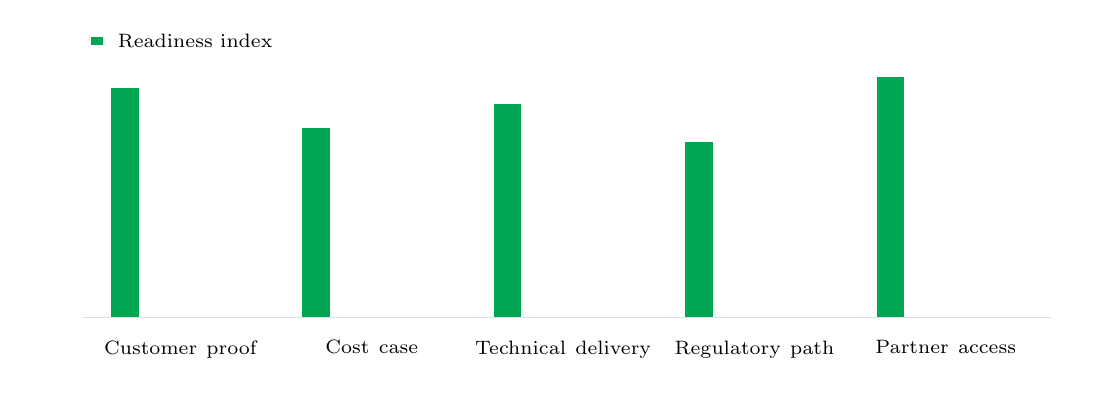
\begin{tikzpicture}[x=1cm,y=1cm]
\path[use as bounding box] (0,0) rectangle (13.20,4.40);
\draw[BOLine] (0.70,0.72) -- (13.00,0.72);
\fill[BOGreen] (1.06,0.72) rectangle (1.41,3.64);
\node[anchor=north,align=center,text width=2.24cm] at (1.94,0.55) {\scriptsize Customer proof};
\fill[BOGreen] (3.49,0.72) rectangle (3.84,3.13);
\node[anchor=north,align=center,text width=2.24cm] at (4.37,0.55) {\scriptsize Cost case};
\fill[BOGreen] (5.92,0.72) rectangle (6.27,3.43);
\node[anchor=north,align=center,text width=2.24cm] at (6.80,0.55) {\scriptsize Technical delivery};
\fill[BOGreen] (8.35,0.72) rectangle (8.70,2.95);
\node[anchor=north,align=center,text width=2.24cm] at (9.23,0.55) {\scriptsize Regulatory path};
\fill[BOGreen] (10.78,0.72) rectangle (11.13,3.77);
\node[anchor=north,align=center,text width=2.24cm] at (11.66,0.55) {\scriptsize Partner access};
\fill[BOGreen] (0.80,4.18) rectangle (0.96,4.28);
\node[anchor=west] at (1.02,4.23) {\scriptsize Readiness index};
\end{tikzpicture}\par\vspace{2pt}
\vspace{1pt}\noindent\begin{minipage}[t]{0.92\linewidth}
{\footnotesize\color{BOText} The exhibit ranks the proof points a CEO should ask teams to close before moving from monitoring to commitment.}\par
\end{minipage}\par\vspace{1pt}
\vspace{4pt}{\footnotesize\color{BOText} The exhibit ranks the proof points a CEO should ask teams to close before moving from monitoring to commitment.}\par
{\scriptsize\color{BOMuted} BlueOcean public-source synthesis.}\par
\vspace{9pt}\textcolor{BOLine}{\rule{\linewidth}{0.3pt}}\vspace{8pt}
{\textcolor{BOGreen}{\scriptsize\bfseries EXHIBIT 2}}\par\vspace{4pt}
{\sffamily\fontsize{17}{21}\selectfont\color{BONavy} Commitment posture should shift as proof matures}\par
{\small\color{BOText} Resource posture for Nuclear Fusion Commercialization Outlook and Strategic Implications}\par\vspace{6pt}
\noindent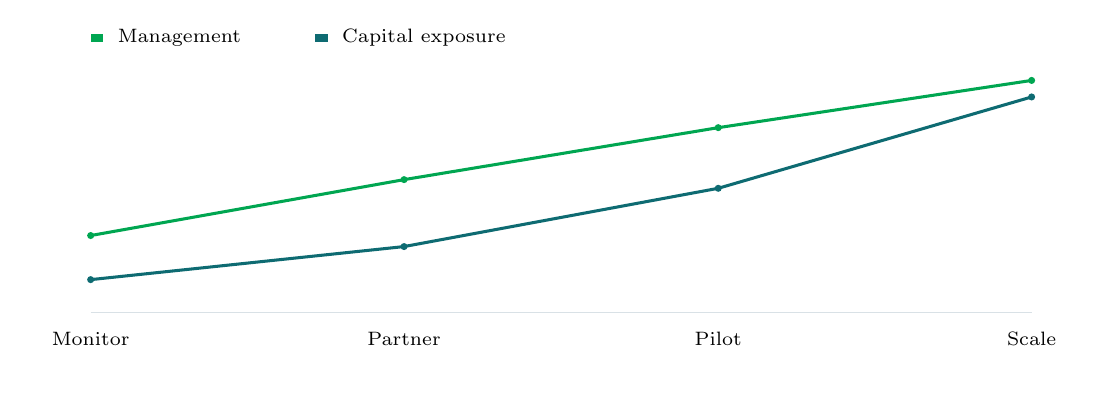
\begin{tikzpicture}[x=1cm,y=1cm]
\path[use as bounding box] (0,0) rectangle (13.20,4.40);
\draw[BOLine] (0.80,0.78) -- (12.75,0.78);
\draw[BOGreen,line width=1.1pt] (0.80,1.76) -- (4.78,2.47) -- (8.77,3.13) -- (12.75,3.73);
\fill[BOGreen] (0.80,1.76) circle (.045);
\fill[BOGreen] (4.78,2.47) circle (.045);
\fill[BOGreen] (8.77,3.13) circle (.045);
\fill[BOGreen] (12.75,3.73) circle (.045);
\draw[BOBlue,line width=1.1pt] (0.80,1.20) -- (4.78,1.62) -- (8.77,2.36) -- (12.75,3.52);
\fill[BOBlue] (0.80,1.20) circle (.045);
\fill[BOBlue] (4.78,1.62) circle (.045);
\fill[BOBlue] (8.77,2.36) circle (.045);
\fill[BOBlue] (12.75,3.52) circle (.045);
\node[anchor=north,align=center,text width=1.8cm] at (0.80,0.66) {\scriptsize Monitor};
\node[anchor=north,align=center,text width=1.8cm] at (4.78,0.66) {\scriptsize Partner};
\node[anchor=north,align=center,text width=1.8cm] at (8.77,0.66) {\scriptsize Pilot};
\node[anchor=north,align=center,text width=1.8cm] at (12.75,0.66) {\scriptsize Scale};
\fill[BOGreen] (0.80,4.22) rectangle (0.96,4.32);
\node[anchor=west] at (1.02,4.27) {\scriptsize Management};
\fill[BOBlue] (3.65,4.22) rectangle (3.81,4.32);
\node[anchor=west] at (3.87,4.27) {\scriptsize Capital exposure};
\end{tikzpicture}\par\vspace{2pt}
\vspace{1pt}\noindent\begin{minipage}[t]{0.92\linewidth}
{\footnotesize\color{BOText} Capital exposure should lag evidence maturity rather than lead it.}\par
\end{minipage}\par\vspace{1pt}
\vspace{4pt}{\footnotesize\color{BOText} Capital exposure should lag evidence maturity rather than lead it.}\par
{\scriptsize\color{BOMuted} BlueOcean scenario synthesis.}\par

\clearpage
{\textcolor{BOGreen}{\scriptsize\bfseries EXHIBIT 3}}\par\vspace{4pt}
{\sffamily\fontsize{17}{21}\selectfont\color{BONavy} Key risks should be ranked by severity and manageability}\par
{\small\color{BOText} Risk exposure for Nuclear Fusion Commercialization Outlook and Strategic Implications}\par\vspace{6pt}
\noindent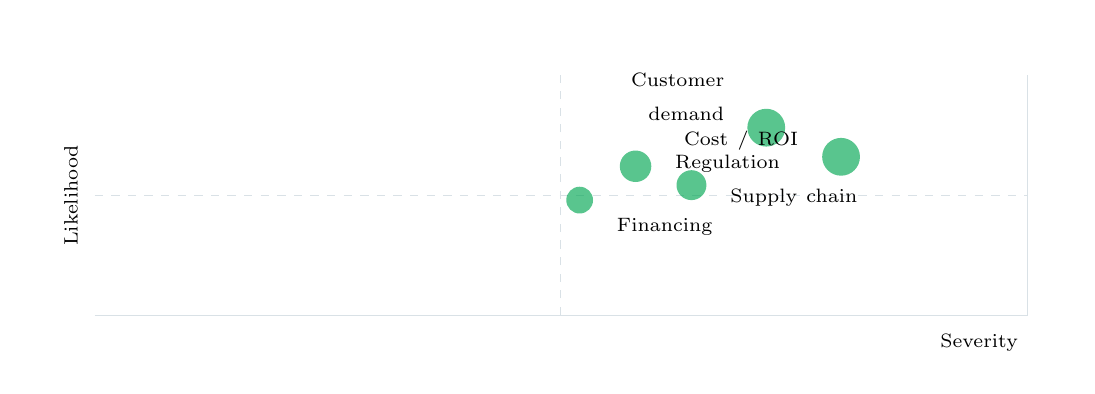
\begin{tikzpicture}[x=1cm,y=1cm]
\path[use as bounding box] (0,0) rectangle (13.20,4.30);
\draw[BOLine] (0.85,0.65) -- (12.70,0.65) -- (12.70,3.70);
\draw[BOLine,dashed] (0.85,2.17) -- (12.70,2.17);
\draw[BOLine,dashed] (6.77,0.65) -- (6.77,3.70);
\fill[BOGreen,opacity=.65] (9.38,3.03) circle (0.24);
\node[anchor=east,align=right,text width=2.10cm] at (8.97,3.42) {\scriptsize Customer demand};
\fill[BOGreen,opacity=.65] (10.33,2.66) circle (0.24);
\node[anchor=east,align=right,text width=2.10cm] at (9.91,2.87) {\scriptsize Cost / ROI};
\fill[BOGreen,opacity=.65] (7.72,2.54) circle (0.20);
\node[anchor=west,align=left,text width=2.10cm] at (8.10,2.57) {\scriptsize Regulation};
\fill[BOGreen,opacity=.65] (8.43,2.30) circle (0.19);
\node[anchor=west,align=left,text width=2.10cm] at (8.80,2.14) {\scriptsize Supply chain};
\fill[BOGreen,opacity=.65] (7.01,2.11) circle (0.17);
\node[anchor=west,align=left,text width=2.10cm] at (7.36,1.77) {\scriptsize Financing};
\node[anchor=north east] at (12.70,0.53) {\scriptsize Severity};
\node[anchor=center,rotate=90] at (0.55,2.17) {\scriptsize Likelihood};
\end{tikzpicture}\par\vspace{2pt}
\vspace{1pt}\noindent\begin{minipage}[t]{0.92\linewidth}
{\footnotesize\color{BOText} Bubble size indicates the management attention required.}\par
\end{minipage}\par\vspace{1pt}
\vspace{4pt}{\footnotesize\color{BOText} Bubble size indicates the management attention required.}\par
{\scriptsize\color{BOMuted} BlueOcean risk screen.}\par
\vspace{9pt}\textcolor{BOLine}{\rule{\linewidth}{0.3pt}}\vspace{8pt}
{\textcolor{BOGreen}{\scriptsize\bfseries EXHIBIT 4}}\par\vspace{4pt}
{\sffamily\fontsize{17}{21}\selectfont\color{BONavy} Diligence workload concentrates in customer, cost and policy proof}\par
{\small\color{BOText} Near-term validation load for Nuclear Fusion Commercialization Outlook and Strategic Implications}\par\vspace{6pt}
\noindent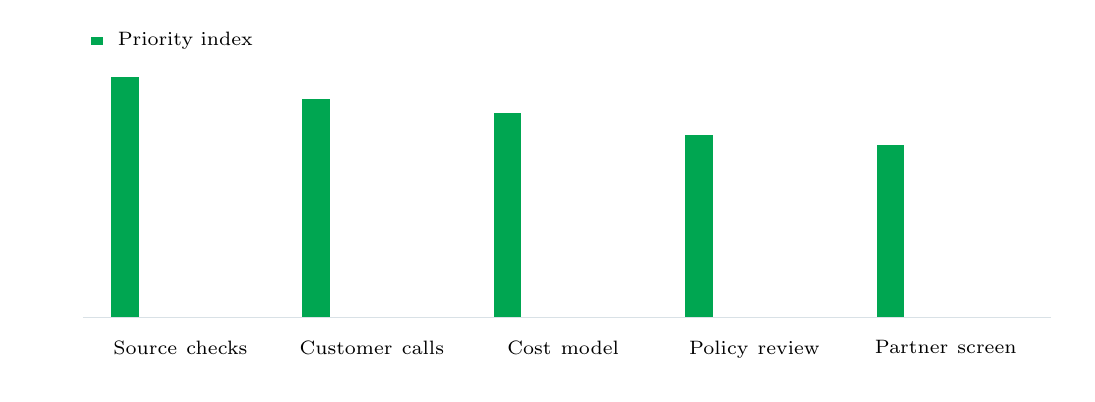
\begin{tikzpicture}[x=1cm,y=1cm]
\path[use as bounding box] (0,0) rectangle (13.20,4.40);
\draw[BOLine] (0.70,0.72) -- (13.00,0.72);
\fill[BOGreen] (1.06,0.72) rectangle (1.41,3.77);
\node[anchor=north,align=center,text width=2.24cm] at (1.94,0.55) {\scriptsize Source checks};
\fill[BOGreen] (3.49,0.72) rectangle (3.84,3.50);
\node[anchor=north,align=center,text width=2.24cm] at (4.37,0.55) {\scriptsize Customer calls};
\fill[BOGreen] (5.92,0.72) rectangle (6.27,3.31);
\node[anchor=north,align=center,text width=2.24cm] at (6.80,0.55) {\scriptsize Cost model};
\fill[BOGreen] (8.35,0.72) rectangle (8.70,3.04);
\node[anchor=north,align=center,text width=2.24cm] at (9.23,0.55) {\scriptsize Policy review};
\fill[BOGreen] (10.78,0.72) rectangle (11.13,2.91);
\node[anchor=north,align=center,text width=2.24cm] at (11.66,0.55) {\scriptsize Partner screen};
\fill[BOGreen] (0.80,4.18) rectangle (0.96,4.28);
\node[anchor=west] at (1.02,4.23) {\scriptsize Priority index};
\end{tikzpicture}\par\vspace{2pt}
\vspace{1pt}\noindent\begin{minipage}[t]{0.92\linewidth}
{\footnotesize\color{BOText} The most valuable work closes open questions that can change the decision.}\par
\end{minipage}\par\vspace{1pt}
\vspace{4pt}{\footnotesize\color{BOText} The most valuable work closes open questions that can change the decision.}\par
{\scriptsize\color{BOMuted} BlueOcean public-source synthesis.}\par

\clearpage
{\textcolor{BOGreen}{\scriptsize\bfseries EXHIBIT 5}}\par\vspace{4pt}
{\sffamily\fontsize{17}{21}\selectfont\color{BONavy} Scenario choices should compare attractiveness with readiness}\par
{\small\color{BOText} Strategic option comparison for Nuclear Fusion Commercialization Outlook and Strategic Implications}\par\vspace{6pt}
{\scriptsize\begin{tabular}{p{38mm}>{\centering\arraybackslash}p{21mm}>{\centering\arraybackslash}p{21mm}>{\centering\arraybackslash}p{21mm}>{\centering\arraybackslash}p{21mm}}
 & {\bfseries Attractiveness} & {\bfseries Readiness} & {\bfseries Confidence} & {\bfseries Capital need} \\
\hline
{\bfseries Fusion Technology Is} & \colorbox{BOGreen}{\textcolor{white}{\strut\hspace{5pt}5\hspace{5pt}}} & \colorbox{BOBlue}{\textcolor{white}{\strut\hspace{5pt}3\hspace{5pt}}} & \colorbox{BOLight}{\textcolor{BOText}{\strut\hspace{5pt}2\hspace{5pt}}} & \colorbox{BOLight}{\textcolor{BOText}{\strut\hspace{5pt}2\hspace{5pt}}} \\
{\bfseries Economic Viability Hinges on} & \colorbox{BOGreen}{\textcolor{white}{\strut\hspace{5pt}4\hspace{5pt}}} & \colorbox{BOGreen}{\textcolor{white}{\strut\hspace{5pt}4\hspace{5pt}}} & \colorbox{BOBlue}{\textcolor{white}{\strut\hspace{5pt}3\hspace{5pt}}} & \colorbox{BOBlue}{\textcolor{white}{\strut\hspace{5pt}3\hspace{5pt}}} \\
{\bfseries Regulatory and Safety} & \colorbox{BOGreen}{\textcolor{white}{\strut\hspace{5pt}4\hspace{5pt}}} & \colorbox{BOLight}{\textcolor{BOText}{\strut\hspace{5pt}2\hspace{5pt}}} & \colorbox{BOLight}{\textcolor{BOText}{\strut\hspace{5pt}2\hspace{5pt}}} & \colorbox{BOGreen}{\textcolor{white}{\strut\hspace{5pt}4\hspace{5pt}}} \\
{\bfseries Nuclear Fusion} & \colorbox{BOBlue}{\textcolor{white}{\strut\hspace{5pt}3\hspace{5pt}}} & \colorbox{BOBlue}{\textcolor{white}{\strut\hspace{5pt}3\hspace{5pt}}} & \colorbox{BOBlue}{\textcolor{white}{\strut\hspace{5pt}3\hspace{5pt}}} & \colorbox{BOLight}{\textcolor{BOText}{\strut\hspace{5pt}2\hspace{5pt}}} \\
{\bfseries Commercial readiness depends on} & \colorbox{BOGreen}{\textcolor{white}{\strut\hspace{5pt}5\hspace{5pt}}} & \colorbox{BOBlue}{\textcolor{white}{\strut\hspace{5pt}3\hspace{5pt}}} & \colorbox{BOBlue}{\textcolor{white}{\strut\hspace{5pt}3\hspace{5pt}}} & \colorbox{BOBlue}{\textcolor{white}{\strut\hspace{5pt}3\hspace{5pt}}} \\
\end{tabular}}\par\vspace{2pt}
\vspace{1pt}\noindent\begin{minipage}[t]{0.92\linewidth}
{\footnotesize\color{BOText} The matrix ranks where the next validation work should focus.}\par
\end{minipage}\par\vspace{1pt}
\vspace{4pt}{\footnotesize\color{BOText} The matrix ranks where the next validation work should focus.}\par
{\scriptsize\color{BOMuted} BlueOcean qualitative assessment.}\par
\vspace{9pt}\textcolor{BOLine}{\rule{\linewidth}{0.3pt}}\vspace{8pt}
{\textcolor{BOGreen}{\scriptsize\bfseries EXHIBIT 6}}\par\vspace{4pt}
{\sffamily\fontsize{17}{21}\selectfont\color{BONavy} Validation effort shifts from customer proof to policy and partners}\par
{\small\color{BOText} Quarterly validation mix for Nuclear Fusion Commercialization Outlook and Strategic Implications}\par\vspace{6pt}
\noindent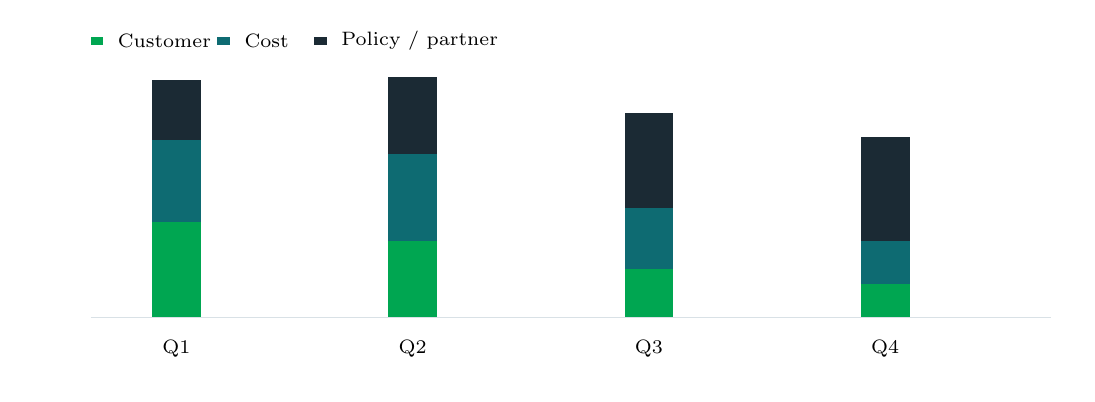
\begin{tikzpicture}[x=1cm,y=1cm]
\path[use as bounding box] (0,0) rectangle (13.20,4.40);
\draw[BOLine] (0.80,0.72) -- (13.00,0.72);
\fill[BOGreen] (1.58,0.72) rectangle (2.20,1.93);
\fill[BOBlue] (1.58,1.93) rectangle (2.20,2.97);
\fill[BONavy] (1.58,2.97) rectangle (2.20,3.74);
\node[anchor=north,align=center,text width=2.76cm] at (1.89,0.55) {\scriptsize Q1};
\fill[BOGreen] (4.58,0.72) rectangle (5.20,1.69);
\fill[BOBlue] (4.58,1.69) rectangle (5.20,2.80);
\fill[BONavy] (4.58,2.80) rectangle (5.20,3.77);
\node[anchor=north,align=center,text width=2.76cm] at (4.89,0.55) {\scriptsize Q2};
\fill[BOGreen] (7.58,0.72) rectangle (8.20,1.34);
\fill[BOBlue] (7.58,1.34) rectangle (8.20,2.11);
\fill[BONavy] (7.58,2.11) rectangle (8.20,3.32);
\node[anchor=north,align=center,text width=2.76cm] at (7.89,0.55) {\scriptsize Q3};
\fill[BOGreen] (10.58,0.72) rectangle (11.20,1.14);
\fill[BOBlue] (10.58,1.14) rectangle (11.20,1.69);
\fill[BONavy] (10.58,1.69) rectangle (11.20,3.01);
\node[anchor=north,align=center,text width=2.76cm] at (10.89,0.55) {\scriptsize Q4};
\fill[BOGreen] (0.80,4.18) rectangle (0.96,4.28);
\node[anchor=west] at (1.02,4.23) {\scriptsize Customer};
\fill[BOBlue] (2.41,4.18) rectangle (2.57,4.28);
\node[anchor=west] at (2.63,4.23) {\scriptsize Cost};
\fill[BONavy] (3.64,4.18) rectangle (3.80,4.28);
\node[anchor=west] at (3.86,4.23) {\scriptsize Policy / partner};
\end{tikzpicture}\par\vspace{2pt}
\vspace{1pt}\noindent\begin{minipage}[t]{0.92\linewidth}
{\footnotesize\color{BOText} The validation cadence should improve facts before escalating resource commitment.}\par
\end{minipage}\par\vspace{1pt}
\vspace{4pt}{\footnotesize\color{BOText} The validation cadence should improve facts before escalating resource commitment.}\par
{\scriptsize\color{BOMuted} BlueOcean public-source synthesis.}\par

\clearpage
{\textcolor{BOGreen}{\scriptsize\bfseries EXHIBIT 7}}\par\vspace{4pt}
{\sffamily\fontsize{17}{21}\selectfont\color{BONavy} Cost structure must be decomposed before underwriting}\par
{\small\color{BOText} Cost diligence view for Nuclear Fusion Commercialization Outlook and Strategic Implications}\par\vspace{6pt}
\noindent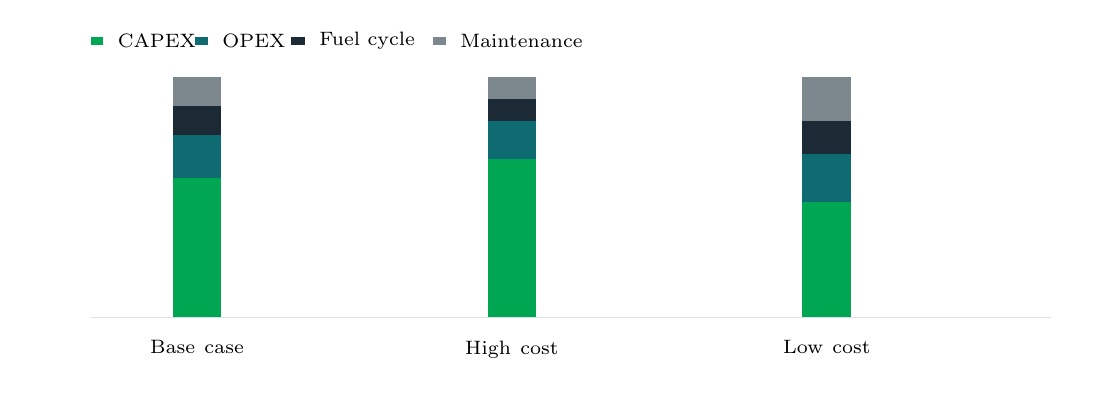
\begin{tikzpicture}[x=1cm,y=1cm]
\path[use as bounding box] (0,0) rectangle (13.20,4.40);
\draw[BOLine] (0.80,0.72) -- (13.00,0.72);
\fill[BOGreen] (1.84,0.72) rectangle (2.46,2.49);
\fill[BOBlue] (1.84,2.49) rectangle (2.46,3.04);
\fill[BONavy] (1.84,3.04) rectangle (2.46,3.40);
\fill[BOMuted] (1.84,3.40) rectangle (2.46,3.77);
\node[anchor=north,align=center,text width=3.68cm] at (2.15,0.55) {\scriptsize Base case};
\fill[BOGreen] (5.84,0.72) rectangle (6.46,2.73);
\fill[BOBlue] (5.84,2.73) rectangle (6.46,3.22);
\fill[BONavy] (5.84,3.22) rectangle (6.46,3.50);
\fill[BOMuted] (5.84,3.50) rectangle (6.46,3.77);
\node[anchor=north,align=center,text width=3.68cm] at (6.15,0.55) {\scriptsize High cost};
\fill[BOGreen] (9.84,0.72) rectangle (10.46,2.18);
\fill[BOBlue] (9.84,2.18) rectangle (10.46,2.79);
\fill[BONavy] (9.84,2.79) rectangle (10.46,3.22);
\fill[BOMuted] (9.84,3.22) rectangle (10.46,3.77);
\node[anchor=north,align=center,text width=3.68cm] at (10.15,0.55) {\scriptsize Low cost};
\fill[BOGreen] (0.80,4.18) rectangle (0.96,4.28);
\node[anchor=west] at (1.02,4.23) {\scriptsize CAPEX};
\fill[BOBlue] (2.12,4.18) rectangle (2.29,4.28);
\node[anchor=west] at (2.35,4.23) {\scriptsize OPEX};
\fill[BONavy] (3.35,4.18) rectangle (3.52,4.28);
\node[anchor=west] at (3.58,4.23) {\scriptsize Fuel cycle};
\fill[BOMuted] (5.15,4.18) rectangle (5.31,4.28);
\node[anchor=west] at (5.37,4.23) {\scriptsize Maintenance};
\end{tikzpicture}\par\vspace{2pt}
\vspace{1pt}\noindent\begin{minipage}[t]{0.92\linewidth}
{\footnotesize\color{BOText} The chart separates capital, operating and maintenance drivers so management can test which cost lever would change the investment case.}\par
\end{minipage}\par\vspace{1pt}
\vspace{4pt}{\footnotesize\color{BOText} The chart separates capital, operating and maintenance drivers so management can test which cost lever would change the investment case.}\par
{\scriptsize\color{BOMuted} BlueOcean public-source synthesis.}\par
\vspace{9pt}\textcolor{BOLine}{\rule{\linewidth}{0.3pt}}\vspace{8pt}
{\textcolor{BOGreen}{\scriptsize\bfseries EXHIBIT 8}}\par\vspace{4pt}
{\sffamily\fontsize{17}{21}\selectfont\color{BONavy} Timeline confidence falls as milestones move from lab to grid}\par
{\small\color{BOText} Milestone confidence for Nuclear Fusion Commercialization Outlook and Strategic Implications}\par\vspace{6pt}
\noindent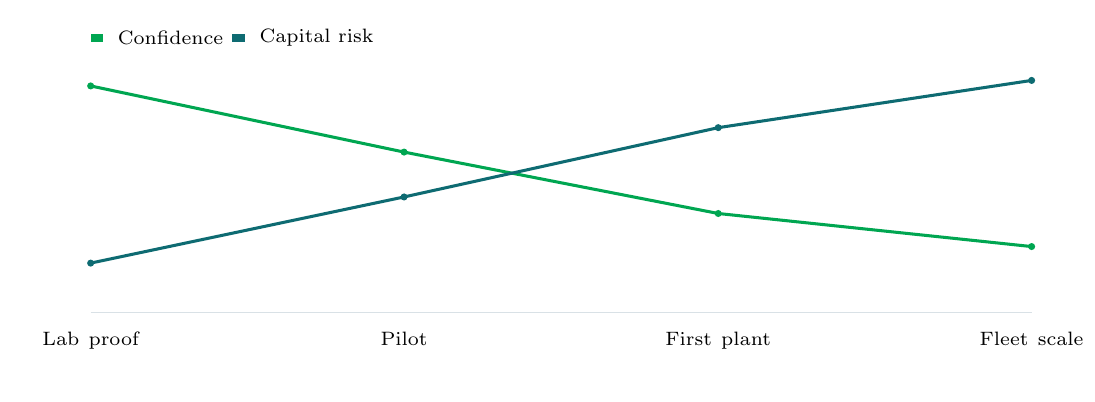
\begin{tikzpicture}[x=1cm,y=1cm]
\path[use as bounding box] (0,0) rectangle (13.20,4.40);
\draw[BOLine] (0.80,0.78) -- (12.75,0.78);
\draw[BOGreen,line width=1.1pt] (0.80,3.66) -- (4.78,2.82) -- (8.77,2.04) -- (12.75,1.62);
\fill[BOGreen] (0.80,3.66) circle (.045);
\fill[BOGreen] (4.78,2.82) circle (.045);
\fill[BOGreen] (8.77,2.04) circle (.045);
\fill[BOGreen] (12.75,1.62) circle (.045);
\draw[BOBlue,line width=1.1pt] (0.80,1.41) -- (4.78,2.25) -- (8.77,3.13) -- (12.75,3.73);
\fill[BOBlue] (0.80,1.41) circle (.045);
\fill[BOBlue] (4.78,2.25) circle (.045);
\fill[BOBlue] (8.77,3.13) circle (.045);
\fill[BOBlue] (12.75,3.73) circle (.045);
\node[anchor=north,align=center,text width=1.8cm] at (0.80,0.66) {\scriptsize Lab proof};
\node[anchor=north,align=center,text width=1.8cm] at (4.78,0.66) {\scriptsize Pilot};
\node[anchor=north,align=center,text width=1.8cm] at (8.77,0.66) {\scriptsize First plant};
\node[anchor=north,align=center,text width=1.8cm] at (12.75,0.66) {\scriptsize Fleet scale};
\fill[BOGreen] (0.80,4.22) rectangle (0.96,4.32);
\node[anchor=west] at (1.02,4.27) {\scriptsize Confidence};
\fill[BOBlue] (2.60,4.22) rectangle (2.76,4.32);
\node[anchor=west] at (2.82,4.27) {\scriptsize Capital risk};
\end{tikzpicture}\par\vspace{2pt}
\vspace{1pt}\noindent\begin{minipage}[t]{0.92\linewidth}
{\footnotesize\color{BOText} Decision confidence should be staged by milestone maturity.}\par
\end{minipage}\par\vspace{1pt}
\vspace{4pt}{\footnotesize\color{BOText} Decision confidence should be staged by milestone maturity.}\par
{\scriptsize\color{BOMuted} BlueOcean milestone assessment.}\par

\clearpage
\label{chap:1}
\noindent\begin{tikzpicture}
\path[use as bounding box] (0,0) rectangle (\linewidth,54mm);
\clip (0,0) rectangle (\linewidth,54mm);
\node[anchor=north west,inner sep=0] at (0,54mm) {
\includegraphics[width=\linewidth]{assets/image-1.png}};
\end{tikzpicture}
\vspace{0pt}
\noindent
\begin{tikzpicture}
\fill[BOGreen] (0,0) rectangle (96mm,1.2pt);
\end{tikzpicture}\par\vspace{8pt}
{\Large\sffamily\bfseries\color{BONavy} Fusion Technology Is Approaching Net Energy Gain, but Commercialization Remains a Decade Away}\par\vspace{4pt}
{\sffamily\fontsize{15}{20}\selectfont\color{BOGreen} The December 2022 fusion ignition at LLNL proves scientific feasibility, but engineering scale-up for commercial power will take at least another decade, requiring sustained investment in plasma confinement, materials, and tritium breeding.}\par\vspace{9pt}
\begin{multicols}{2}
{\small The December 2022 achievement of fusion ignition at Lawrence Livermore National Laboratory marked a historic scientific milestone: for the first time, a controlled fusion experiment produced more energy than the laser energy used to drive it, delivering 2.15 MJ of fusion energy output. This breakthrough, decades in the making, has shifted the narrative from \BOApos{}always 30 years away\BOApos{} to a more tangible timeline. However, this was a single-shot inertial confinement experiment, not a sustained power plant. The path to commercial fusion requires solving multiple engineering challenges, including plasma confinement, materials that can withstand extreme neutron fluxes, and tritium breeding.}\par
{\small Multiple private companies are pursuing different reactor designs. Commonwealth Fusion Systems is building SPARC, a compact tokamak aiming for net energy gain by 2025-2027. TAE Technologies is developing a field-reversed configuration approach. Helion Energy is targeting a pulsed fusion system with direct electricity conversion. These companies have attracted significant private investment, with over \$5 billion raised collectively since 2020. However, historical fusion projects like ITER have experienced decades of delays and cost overruns. ITER, the international tokamak project, is now expected to achieve first plasma in 2025 and full fusion power in 2035, but its budget has ballooned to over \$20 billion.}\par
{\small The key technical hurdles are well-documented. Plasma confinement requires maintaining temperatures over 100 million degrees Celsius while preventing instabilities. Materials must withstand high-energy neutrons that can degrade structural integrity. Tritium breeding is essential for fuel self-sufficiency, but no breeding blanket has been demonstrated at scale. These challenges are being addressed through advanced simulations, new materials like high-temperature superconductors, and public-private partnerships. The U.S. Department of Energy\BOApos{}s Fusion Energy Sciences program supports a roadmap to \BOApos{}Build, Innovate, and Grow\BOApos{} a domestic fusion industry.}\par
{\small Timeline estimates vary widely. Optimistic projections from private firms suggest pilot plants by the early 2030s, but independent assessments, such as the National Academies study \BOApos{}Bringing Fusion to the U.S. Grid,\BOApos{} indicate that commercial fusion electricity is unlikely before 2040-2050. The gap between scientific breakeven and commercial viability is substantial, requiring scale-up by factors of 10-100 in energy output and reliability. Investors should expect delays and cost overruns, but the direction of travel is clear: fusion is no longer a theoretical possibility but an engineering challenge.}\par
{\small For decision-makers, the key implication is that fusion is a long-term play. Early investment in enabling technologies (superconductors, lasers, tritium breeding) can provide returns before full-scale reactors are built. Companies that secure supply chain positions now will be well-placed when the technology matures. The risk of over-investing in hype is real, but the cost of missing a transformative technology is higher.}\par
{\small In summary, fusion technology has crossed a critical threshold, but the road to commercialization is long and uncertain. A disciplined, milestone-based approach to investment and partnership is essential to capture upside while managing downside risk.}\par
{\small For leadership, Nuclear Fusion Commercialization Outlook and Strategic Implications should be separated into near-term actions, option-building moves and commitments that require stronger proof. That distinction keeps market enthusiasm or technical narrative from becoming an investment conclusion too early.}\par
\end{multicols}
\label{chap:1:end}

\clearpage
\label{chap:2}
\noindent\begin{tikzpicture}
\path[use as bounding box] (0,0) rectangle (\linewidth,54mm);
\clip (0,0) rectangle (\linewidth,54mm);
\node[anchor=north west,inner sep=0] at (0,54mm) {
\includegraphics[width=\linewidth]{assets/image-2.png}};
\end{tikzpicture}
\vspace{0pt}
\noindent
\begin{tikzpicture}
\fill[BOGreen] (0,0) rectangle (96mm,1.2pt);
\end{tikzpicture}\par\vspace{8pt}
{\Large\sffamily\bfseries\color{BONavy} Economic Viability Hinges on Cost Reductions and Scale-Up, with LCOE Uncertain vs. Renewables}\par\vspace{4pt}
{\sffamily\fontsize{15}{20}\selectfont\color{BOGreen} Fusion\BOApos{}s LCOE projections (\$50-100+/MWh by 2050) face stiff competition from rapidly falling solar and wind costs (<\$30/MWh today), making fusion\BOApos{}s economic case dependent on carbon pricing or niche applications like industrial heat.}\par\vspace{9pt}
\begin{multicols}{2}
{\small The levelized cost of electricity (LCOE) for fusion is highly uncertain, with projections ranging from \$50/MWh to over \$100/MWh by 2050, depending on capital costs, capacity factors, and fuel costs. In contrast, solar and wind LCOE have already fallen below \$30/MWh in many regions and continue to decline with storage costs. This raises a fundamental question: can fusion ever compete on cost for bulk electricity generation?}\par
{\small Fusion\BOApos{}s capital costs are expected to be high due to complex reactor systems, including superconducting magnets, vacuum vessels, and tritium breeding blankets. A typical 1 GW fusion plant might cost \$5-10 billion, similar to fission plants. However, fusion fuel (deuterium and lithium) is abundant and cheap, leading to low variable costs. If fusion plants can achieve high capacity factors (90\%+), they could provide baseload power at competitive rates, especially if carbon pricing is implemented.}\par
{\small But the rapid decline of renewables and storage is a moving target. Solar-plus-storage LCOE is projected to fall below \$20/MWh by 2030 in sunny regions, making it difficult for any new baseload technology to compete. Fusion\BOApos{}s value proposition may therefore lie in applications where renewables are less effective: industrial heat (e.g., steel, cement), hydrogen production, and remote or off-grid locations. These markets are smaller but could offer higher margins.}\par
{\small Market size scenarios depend on policy and technology. In a high-decarbonization scenario with strong carbon pricing, fusion could capture 10-20\% of global electricity by 2050, representing a multi-trillion-dollar market. In a low-carbon-pricing scenario, fusion may be limited to niche applications. The key uncertainty is the pace of renewable cost declines and the availability of long-duration storage.}\par
{\small Investment in fusion should therefore be viewed as a long-term hedge with asymmetric upside. Early movers in the supply chain-such as manufacturers of high-temperature superconductors, advanced lasers, and tritium breeding components-may capture value even if reactor deployment is delayed. The strategic question is not whether fusion will work, but when and at what cost.}\par
{\small A practical reading is that the bottom line is that fusion\BOApos{}s economic viability is not guaranteed. A portfolio approach that includes both fusion and other clean energy technologies is prudent. Companies should prepare for multiple scenarios, including one where fusion never achieves cost parity with renewables.}\par
{\small Commercial readiness should be judged through customer adoption, cost structure, delivery cycle, service capability and financing availability. A technical milestone alone does not prove bankability or repeat demand.}\par
\end{multicols}
\label{chap:2:end}

\clearpage
{\textcolor{BOGreen}{\scriptsize\bfseries EXHIBIT 9}}\par\vspace{4pt}
{\sffamily\fontsize{17}{21}\selectfont\color{BONavy} Partner options differ on learning value and capital exposure}\par
{\small\color{BOText} Where-to-play option view for Nuclear Fusion Commercialization Outlook and Strategic Implications}\par\vspace{6pt}
{\scriptsize\begin{tabular}{p{38mm}>{\centering\arraybackslash}p{21mm}>{\centering\arraybackslash}p{21mm}>{\centering\arraybackslash}p{21mm}>{\centering\arraybackslash}p{21mm}}
 & {\bfseries Learning} & {\bfseries Control} & {\bfseries Capital need} & {\bfseries Reversibility} \\
\hline
{\bfseries Direct equity} & \colorbox{BOGreen}{\textcolor{white}{\strut\hspace{5pt}5\hspace{5pt}}} & \colorbox{BOGreen}{\textcolor{white}{\strut\hspace{5pt}4\hspace{5pt}}} & \colorbox{BOLight}{\textcolor{BOText}{\strut\hspace{5pt}2\hspace{5pt}}} & \colorbox{BOLight}{\textcolor{BOText}{\strut\hspace{5pt}2\hspace{5pt}}} \\
{\bfseries Corporate venture} & \colorbox{BOGreen}{\textcolor{white}{\strut\hspace{5pt}4\hspace{5pt}}} & \colorbox{BOBlue}{\textcolor{white}{\strut\hspace{5pt}3\hspace{5pt}}} & \colorbox{BOBlue}{\textcolor{white}{\strut\hspace{5pt}3\hspace{5pt}}} & \colorbox{BOBlue}{\textcolor{white}{\strut\hspace{5pt}3\hspace{5pt}}} \\
{\bfseries Offtake option} & \colorbox{BOBlue}{\textcolor{white}{\strut\hspace{5pt}3\hspace{5pt}}} & \colorbox{BOLight}{\textcolor{BOText}{\strut\hspace{5pt}2\hspace{5pt}}} & \colorbox{BOGreen}{\textcolor{white}{\strut\hspace{5pt}4\hspace{5pt}}} & \colorbox{BOGreen}{\textcolor{white}{\strut\hspace{5pt}4\hspace{5pt}}} \\
{\bfseries Supplier JV} & \colorbox{BOGreen}{\textcolor{white}{\strut\hspace{5pt}4\hspace{5pt}}} & \colorbox{BOGreen}{\textcolor{white}{\strut\hspace{5pt}4\hspace{5pt}}} & \colorbox{BOLight}{\textcolor{BOText}{\strut\hspace{5pt}2\hspace{5pt}}} & \colorbox{BOLight}{\textcolor{BOText}{\strut\hspace{5pt}2\hspace{5pt}}} \\
{\bfseries R\&D consortium} & \colorbox{BOBlue}{\textcolor{white}{\strut\hspace{5pt}3\hspace{5pt}}} & \colorbox{BOLight}{\textcolor{BOText}{\strut\hspace{5pt}2\hspace{5pt}}} & \colorbox{BOGreen}{\textcolor{white}{\strut\hspace{5pt}5\hspace{5pt}}} & \colorbox{BOGreen}{\textcolor{white}{\strut\hspace{5pt}5\hspace{5pt}}} \\
\end{tabular}}\par\vspace{2pt}
\vspace{1pt}\noindent\begin{minipage}[t]{0.92\linewidth}
{\footnotesize\color{BOText} The best early posture maximizes learning without forcing irreversible capital exposure.}\par
\end{minipage}\par\vspace{1pt}
\vspace{4pt}{\footnotesize\color{BOText} The best early posture maximizes learning without forcing irreversible capital exposure.}\par
{\scriptsize\color{BOMuted} BlueOcean option synthesis.}\par
\vspace{9pt}\textcolor{BOLine}{\rule{\linewidth}{0.3pt}}\vspace{8pt}
{\textcolor{BOGreen}{\scriptsize\bfseries EXHIBIT 10}}\par\vspace{4pt}
{\sffamily\fontsize{17}{21}\selectfont\color{BONavy} Evidence maturity varies sharply by claim type}\par
{\small\color{BOText} Claim maturity for Nuclear Fusion Commercialization Outlook and Strategic Implications}\par\vspace{6pt}
\noindent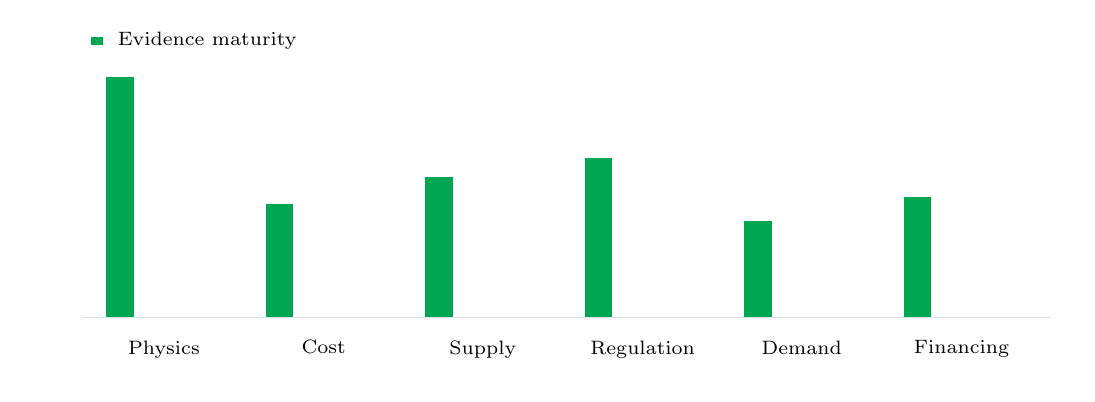
\begin{tikzpicture}[x=1cm,y=1cm]
\path[use as bounding box] (0,0) rectangle (13.20,4.40);
\draw[BOLine] (0.70,0.72) -- (13.00,0.72);
\fill[BOGreen] (1.00,0.72) rectangle (1.35,3.77);
\node[anchor=north,align=center,text width=1.86cm] at (1.73,0.55) {\scriptsize Physics};
\fill[BOGreen] (3.03,0.72) rectangle (3.37,2.16);
\node[anchor=north,align=center,text width=1.86cm] at (3.76,0.55) {\scriptsize Cost};
\fill[BOGreen] (5.05,0.72) rectangle (5.40,2.50);
\node[anchor=north,align=center,text width=1.86cm] at (5.78,0.55) {\scriptsize Supply};
\fill[BOGreen] (7.08,0.72) rectangle (7.42,2.75);
\node[anchor=north,align=center,text width=1.86cm] at (7.81,0.55) {\scriptsize Regulation};
\fill[BOGreen] (9.10,0.72) rectangle (9.45,1.95);
\node[anchor=north,align=center,text width=1.86cm] at (9.83,0.55) {\scriptsize Demand};
\fill[BOGreen] (11.13,0.72) rectangle (11.47,2.25);
\node[anchor=north,align=center,text width=1.86cm] at (11.86,0.55) {\scriptsize Financing};
\fill[BOGreen] (0.80,4.18) rectangle (0.96,4.28);
\node[anchor=west] at (1.02,4.23) {\scriptsize Evidence maturity};
\end{tikzpicture}\par\vspace{2pt}
\vspace{1pt}\noindent\begin{minipage}[t]{0.92\linewidth}
{\footnotesize\color{BOText} Management can use the maturity gap to decide which claims support action today and which require a separate diligence workstream.}\par
\end{minipage}\par\vspace{1pt}
\vspace{4pt}{\footnotesize\color{BOText} Management can use the maturity gap to decide which claims support action today and which require a separate diligence workstream.}\par
{\scriptsize\color{BOMuted} BlueOcean public-source synthesis.}\par

\clearpage
\label{chap:3}
\noindent\begin{tikzpicture}
\path[use as bounding box] (0,0) rectangle (\linewidth,54mm);
\clip (0,0) rectangle (\linewidth,54mm);
\node[anchor=north west,inner sep=0] at (0,54mm) {
\includegraphics[width=\linewidth]{assets/image-3.png}};
\end{tikzpicture}
\vspace{0pt}
\noindent
\begin{tikzpicture}
\fill[BOGreen] (0,0) rectangle (96mm,1.2pt);
\end{tikzpicture}\par\vspace{8pt}
{\Large\sffamily\bfseries\color{BONavy} Regulatory and Safety Frameworks Are Nascent but Critical for Public Acceptance}\par\vspace{4pt}
{\sffamily\fontsize{15}{20}\selectfont\color{BOGreen} Fusion\BOApos{}s regulatory path is still being defined (U.S. NRC proposed rule in 2023), and while fusion produces less long-lived waste than fission, tritium containment and public perception remain key risks that require proactive engagement.}\par\vspace{9pt}
\begin{multicols}{2}
{\small Fusion energy produces less long-lived radioactive waste than fission, as the primary structural materials become activated but decay to safe levels within decades. However, fusion still requires robust safety and waste management regulations. The U.S. Nuclear Regulatory Commission (NRC) is developing a licensing framework for fusion, but it is not yet finalized. In 2023, the NRC issued a proposed rule that would regulate fusion similarly to particle accelerators rather than fission reactors, which could streamline licensing. However, public perception may still conflate fusion with fission, requiring proactive communication.}\par
{\small Internationally, the ITER project is providing valuable experience in regulatory compliance for a fusion facility. ITER is licensed under French nuclear regulations, which have been adapted for fusion. This precedent may inform future licensing for commercial plants. However, each country will develop its own framework, leading to potential fragmentation.}\par
{\small Safety risks include tritium leakage, which is radioactive and can be incorporated into water. Tritium is difficult to contain due to its small size and mobility. Fusion plants will require multiple containment barriers and monitoring systems. The risk of a runaway reaction is minimal because fusion plasmas are inherently unstable and will shut down if conditions deviate.}\par
{\small Waste management is a key advantage: fusion does not produce high-level radioactive waste like fission spent fuel. The activated materials can be recycled or disposed of in near-surface repositories after a few decades. This could reduce public opposition compared to fission. However, the lack of a long-term waste solution for fission has been a major barrier; fusion must avoid similar pitfalls.}\par
{\small Public acceptance will depend on safety records, waste management plans, and perceived benefits. Early engagement with communities and transparent communication are essential. Fusion\BOApos{}s potential to provide clean, abundant energy could generate strong public support, but any accidents or regulatory failures could set back the industry by decades.}\par
{\small For leadership teams, for decision-makers, the key is to engage early with regulators and invest in safety design. Companies that help shape the regulatory framework will have a competitive advantage. Public perception should be managed through clear communication about fusion\BOApos{}s safety and waste advantages over fission.}\par
{\small Every opportunity eventually returns to cost, revenue, margin, cash flow and timing. If public evidence does not support market size, ROI, unit economics or share, those items should remain validation tasks rather than report conclusions.}\par
\end{multicols}
\label{chap:3:end}

\clearpage
\label{chap:4}
\noindent\begin{tikzpicture}
\path[use as bounding box] (0,0) rectangle (\linewidth,54mm);
\clip (0,0) rectangle (\linewidth,54mm);
\node[anchor=north west,inner sep=0] at (0,54mm) {
\includegraphics[width=\linewidth]{assets/image-4.png}};
\end{tikzpicture}
\vspace{0pt}
\noindent
\begin{tikzpicture}
\fill[BOGreen] (0,0) rectangle (96mm,1.2pt);
\end{tikzpicture}\par\vspace{8pt}
{\Large\sffamily\bfseries\color{BONavy} Nuclear Fusion Commercialization Outlook and Strategic Implications should be managed as a staged strategic option, not a binary bet}\par\vspace{4pt}
{\sffamily\fontsize{15}{20}\selectfont\color{BOGreen} The CEO question is which moves are safe now and which should wait for stronger evidence.}\par\vspace{9pt}
\begin{multicols}{2}
{\small The operating takeaway is that for leadership, Nuclear Fusion Commercialization Outlook and Strategic Implications should be separated into near-term actions, option-building moves and commitments that require stronger proof. That distinction keeps market enthusiasm or technical narrative from becoming an investment conclusion too early.}\par
{\small From a board perspective, the immediate management question is not whether the opportunity is exciting; it is whether budget, partner access or management attention should be committed now. Low-cost validation can start early, while larger capital commitments should wait for customer, cost, financing, regulatory or operating proof.}\par
{\small The current evidence posture is: Public-evidence signal: [Source 1: U.S. DOE Fusion Energy Sciences] The Department of Energy has been a leader in fusion energy research since the 1950s and supports groundbreaking advances today. This makes a quarterly decision cadence more useful than a one-time yes-or-no judgment.}\par
{\small For a CEO, Nuclear Fusion Commercialization Outlook and Strategic Implications should be managed as a staged strategic option, not. matters only if it changes the timing of capital, partner access, customer commitments or risk appetite. The strongest posture is to keep learning close to the business while reserving heavier commitments for proof that can survive investment-committee scrutiny.}\par
{\small For Nuclear Fusion Commercialization Outlook and Strategic Implications should be managed as a staged strategic option, not., resource allocation should follow the facts that can change the decision: customer demand, cost position, financing availability, regulatory path and delivery capability. If those facts do not improve, increasing exposure mainly creates strategic lock-in rather than higher conviction.}\par
{\small The public record on Nuclear Fusion Commercialization Outlook and Strategic Implications should be managed as a staged strategic option, not. provides a starting point, not a complete underwriting case. The most useful retained signal is: [Source 1: U.S. DOE Fusion Energy Sciences] The Department of Energy has been a leader in fusion energy research since the 1950s and supports groundbreaking advances today. Management should turn that signal into explicit diligence questions rather than a broader claim.}\par
\end{multicols}
\label{chap:4:end}

\clearpage
{\textcolor{BOGreen}{\scriptsize\bfseries EXHIBIT 11}}\par\vspace{4pt}
{\sffamily\fontsize{17}{21}\selectfont\color{BONavy} Use-case priorities separate early revenue from long-term optionality}\par
{\small\color{BOText} Customer option screen for Nuclear Fusion Commercialization Outlook and Strategic Implications}\par\vspace{6pt}
{\scriptsize\begin{tabular}{p{38mm}>{\centering\arraybackslash}p{21mm}>{\centering\arraybackslash}p{21mm}>{\centering\arraybackslash}p{21mm}>{\centering\arraybackslash}p{21mm}}
 & {\bfseries Demand pull} & {\bfseries Price tolerance} & {\bfseries Timing} & {\bfseries Evidence} \\
\hline
{\bfseries Industrial heat} & \colorbox{BOGreen}{\textcolor{white}{\strut\hspace{5pt}5\hspace{5pt}}} & \colorbox{BOGreen}{\textcolor{white}{\strut\hspace{5pt}4\hspace{5pt}}} & \colorbox{BOBlue}{\textcolor{white}{\strut\hspace{5pt}3\hspace{5pt}}} & \colorbox{BOBlue}{\textcolor{white}{\strut\hspace{5pt}3\hspace{5pt}}} \\
{\bfseries Hydrogen} & \colorbox{BOGreen}{\textcolor{white}{\strut\hspace{5pt}4\hspace{5pt}}} & \colorbox{BOGreen}{\textcolor{white}{\strut\hspace{5pt}4\hspace{5pt}}} & \colorbox{BOBlue}{\textcolor{white}{\strut\hspace{5pt}3\hspace{5pt}}} & \colorbox{BOLight}{\textcolor{BOText}{\strut\hspace{5pt}2\hspace{5pt}}} \\
{\bfseries Grid power} & \colorbox{BOGreen}{\textcolor{white}{\strut\hspace{5pt}5\hspace{5pt}}} & \colorbox{BOLight}{\textcolor{BOText}{\strut\hspace{5pt}2\hspace{5pt}}} & \colorbox{BOLight}{\textcolor{BOText}{\strut\hspace{5pt}1\hspace{5pt}}} & \colorbox{BOLight}{\textcolor{BOText}{\strut\hspace{5pt}2\hspace{5pt}}} \\
{\bfseries Defense / remote} & \colorbox{BOBlue}{\textcolor{white}{\strut\hspace{5pt}3\hspace{5pt}}} & \colorbox{BOGreen}{\textcolor{white}{\strut\hspace{5pt}5\hspace{5pt}}} & \colorbox{BOBlue}{\textcolor{white}{\strut\hspace{5pt}3\hspace{5pt}}} & \colorbox{BOLight}{\textcolor{BOText}{\strut\hspace{5pt}2\hspace{5pt}}} \\
{\bfseries Research services} & \colorbox{BOLight}{\textcolor{BOText}{\strut\hspace{5pt}2\hspace{5pt}}} & \colorbox{BOBlue}{\textcolor{white}{\strut\hspace{5pt}3\hspace{5pt}}} & \colorbox{BOGreen}{\textcolor{white}{\strut\hspace{5pt}4\hspace{5pt}}} & \colorbox{BOGreen}{\textcolor{white}{\strut\hspace{5pt}4\hspace{5pt}}} \\
\end{tabular}}\par\vspace{2pt}
\vspace{1pt}\noindent\begin{minipage}[t]{0.92\linewidth}
{\footnotesize\color{BOText} The comparison separates markets that can teach the company soon from markets that may require longer proof cycles.}\par
\end{minipage}\par\vspace{1pt}
\vspace{4pt}{\footnotesize\color{BOText} The comparison separates markets that can teach the company soon from markets that may require longer proof cycles.}\par
{\scriptsize\color{BOMuted} BlueOcean customer option synthesis.}\par
\vspace{9pt}\textcolor{BOLine}{\rule{\linewidth}{0.3pt}}\vspace{8pt}
{\textcolor{BOGreen}{\scriptsize\bfseries EXHIBIT 12}}\par\vspace{4pt}
{\sffamily\fontsize{17}{21}\selectfont\color{BONavy} Capital exposure should be staged by decision milestone}\par
{\small\color{BOText} Commitment profile for Nuclear Fusion Commercialization Outlook and Strategic Implications}\par\vspace{6pt}
\noindent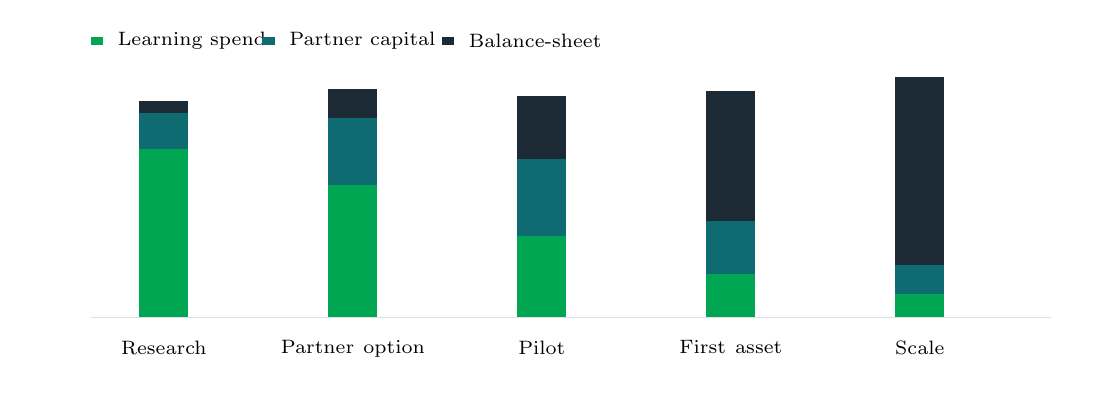
\begin{tikzpicture}[x=1cm,y=1cm]
\path[use as bounding box] (0,0) rectangle (13.20,4.40);
\draw[BOLine] (0.80,0.72) -- (13.00,0.72);
\fill[BOGreen] (1.42,0.72) rectangle (2.04,2.86);
\fill[BOBlue] (1.42,2.86) rectangle (2.04,3.31);
\fill[BONavy] (1.42,3.31) rectangle (2.04,3.47);
\node[anchor=north,align=center,text width=2.21cm] at (1.73,0.55) {\scriptsize Research};
\fill[BOGreen] (3.82,0.72) rectangle (4.44,2.40);
\fill[BOBlue] (3.82,2.40) rectangle (4.44,3.25);
\fill[BONavy] (3.82,3.25) rectangle (4.44,3.62);
\node[anchor=north,align=center,text width=2.21cm] at (4.13,0.55) {\scriptsize Partner option};
\fill[BOGreen] (6.22,0.72) rectangle (6.84,1.76);
\fill[BOBlue] (6.22,1.76) rectangle (6.84,2.73);
\fill[BONavy] (6.22,2.73) rectangle (6.84,3.53);
\node[anchor=north,align=center,text width=2.21cm] at (6.53,0.55) {\scriptsize Pilot};
\fill[BOGreen] (8.62,0.72) rectangle (9.24,1.27);
\fill[BOBlue] (8.62,1.27) rectangle (9.24,1.94);
\fill[BONavy] (8.62,1.94) rectangle (9.24,3.59);
\node[anchor=north,align=center,text width=2.21cm] at (8.93,0.55) {\scriptsize First asset};
\fill[BOGreen] (11.02,0.72) rectangle (11.64,1.02);
\fill[BOBlue] (11.02,1.02) rectangle (11.64,1.39);
\fill[BONavy] (11.02,1.39) rectangle (11.64,3.77);
\node[anchor=north,align=center,text width=2.21cm] at (11.33,0.55) {\scriptsize Scale};
\fill[BOGreen] (0.80,4.18) rectangle (0.96,4.28);
\node[anchor=west] at (1.02,4.23) {\scriptsize Learning spend};
\fill[BOBlue] (2.98,4.18) rectangle (3.14,4.28);
\node[anchor=west] at (3.20,4.23) {\scriptsize Partner capital};
\fill[BONavy] (5.26,4.18) rectangle (5.42,4.28);
\node[anchor=west] at (5.48,4.23) {\scriptsize Balance-sheet};
\end{tikzpicture}\par\vspace{2pt}
\vspace{1pt}\noindent\begin{minipage}[t]{0.92\linewidth}
{\footnotesize\color{BOText} The capital mix should move from learning to committed exposure only as evidence matures.}\par
\end{minipage}\par\vspace{1pt}
\vspace{4pt}{\footnotesize\color{BOText} The capital mix should move from learning to committed exposure only as evidence matures.}\par
{\scriptsize\color{BOMuted} BlueOcean capital staging view.}\par

\clearpage
\label{chap:5}
\noindent\begin{tikzpicture}
\path[use as bounding box] (0,0) rectangle (\linewidth,54mm);
\clip (0,0) rectangle (\linewidth,54mm);
\node[anchor=north west,inner sep=0] at (0,54mm) {
\includegraphics[width=\linewidth]{assets/image-5.png}};
\end{tikzpicture}
\vspace{0pt}
\noindent
\begin{tikzpicture}
\fill[BOGreen] (0,0) rectangle (96mm,1.2pt);
\end{tikzpicture}\par\vspace{8pt}
{\Large\sffamily\bfseries\color{BONavy} Commercial readiness depends on bankability, deliverability and repeat customer proof}\par\vspace{4pt}
{\sffamily\fontsize{15}{20}\selectfont\color{BOGreen} Technical feasibility matters only when it changes customer value, cost position and execution confidence.}\par\vspace{9pt}
\begin{multicols}{2}
{\small From a board perspective, commercial readiness should be judged through customer adoption, cost structure, delivery cycle, service capability and financing availability. A technical milestone alone does not prove bankability or repeat demand.}\par
{\small The commercial implication is that management should require every major assumption to tie back to a verifiable claim: target customer, buying trigger, budget owner, substitute, use case and payback path. Where public evidence is missing, keep the claim directional.}\par
{\small A more robust path is to build credible proof through pilots, partner diligence and third-party validation before moving into larger commitments.}\par
{\small For a CEO, Commercial readiness depends on bankability, deliverability and repeat customer proof matters only if it changes the timing of capital, partner access, customer commitments or risk appetite. The strongest posture is to keep learning close to the business while reserving heavier commitments for proof that can survive investment-committee scrutiny.}\par
{\small For Commercial readiness depends on bankability, deliverability and repeat customer proof, resource allocation should follow the facts that can change the decision: customer demand, cost position, financing availability, regulatory path and delivery capability. If those facts do not improve, increasing exposure mainly creates strategic lock-in rather than higher conviction.}\par
{\small The decision lens is that the public record on Commercial readiness depends on bankability, deliverability and repeat customer proof provides a starting point, not a complete underwriting case. The most useful retained signal is: [Source 1: U.S. DOE Fusion Energy Sciences] The Department of Energy has been a leader in fusion energy research since the 1950s and supports groundbreaking advances today. Management should turn that signal into explicit diligence questions rather than a broader claim.}\par
{\small Where Commercial readiness depends on bankability, deliverability and repeat customer proof depends on numbers, the next review should focus on [Source 1: U.S. DOE Fusion Energy Sciences] The Department of Energy has been a leader in fusion energy research since the 1950s and supports groundbreaking advances today.. Those figures determine whether the opportunity belongs in budget planning, option building or continued monitoring.}\par
\end{multicols}
\label{chap:5:end}

\clearpage
\label{chap:6}
\noindent\begin{tikzpicture}
\path[use as bounding box] (0,0) rectangle (\linewidth,54mm);
\clip (0,0) rectangle (\linewidth,54mm);
\node[anchor=north west,inner sep=0] at (0,54mm) {
\includegraphics[width=\linewidth]{assets/image-6.png}};
\end{tikzpicture}
\vspace{0pt}
\noindent
\begin{tikzpicture}
\fill[BOGreen] (0,0) rectangle (96mm,1.2pt);
\end{tikzpicture}\par\vspace{8pt}
{\Large\sffamily\bfseries\color{BONavy} Cost, return and timing will determine the real deployment window}\par\vspace{4pt}
{\sffamily\fontsize{15}{20}\selectfont\color{BOGreen} Market size should not enter an investment case until the cost and return logic can be checked.}\par\vspace{9pt}
\begin{multicols}{2}
{\small The commercial implication is that every opportunity eventually returns to cost, revenue, margin, cash flow and timing. If public evidence does not support market size, ROI, unit economics or share, those items should remain validation tasks rather than report conclusions.}\par
{\small The board-level question is whether near-term action should focus on verifiable cost drivers and customer willingness to pay instead of relying on optimistic long-range scenarios. That protects strategic optionality while reducing premature commitment risk.}\par
{\small As cost, customer and financing evidence improves, management can shift resources from monitoring and partnerships toward pilots or scaled deployment.}\par
{\small For a CEO, Cost, return and timing will determine the real deployment window matters only if it changes the timing of capital, partner access, customer commitments or risk appetite. The strongest posture is to keep learning close to the business while reserving heavier commitments for proof that can survive investment-committee scrutiny.}\par
{\small For Cost, return and timing will determine the real deployment window, resource allocation should follow the facts that can change the decision: customer demand, cost position, financing availability, regulatory path and delivery capability. If those facts do not improve, increasing exposure mainly creates strategic lock-in rather than higher conviction.}\par
{\small For capital allocation, the public record on Cost, return and timing will determine the real deployment window provides a starting point, not a complete underwriting case. The most useful retained signal is: [Source 1: U.S. DOE Fusion Energy Sciences] The Department of Energy has been a leader in fusion energy research since the 1950s and supports groundbreaking advances today. Management should turn that signal into explicit diligence questions rather than a broader claim.}\par
{\small Where Cost, return and timing will determine the real deployment window depends on numbers, the next review should focus on [Source 1: U.S. DOE Fusion Energy Sciences] The Department of Energy has been a leader in fusion energy research since the 1950s and supports groundbreaking advances today.. Those figures determine whether the opportunity belongs in budget planning, option building or continued monitoring.}\par
\end{multicols}
\label{chap:6:end}

\clearpage
{\textcolor{BOGreen}{\scriptsize\bfseries EXHIBIT 13}}\par\vspace{4pt}
{\sffamily\fontsize{17}{21}\selectfont\color{BONavy} Management attention shifts as the uncertainty stack resolves}\par
{\small\color{BOText} Executive review cadence for Nuclear Fusion Commercialization Outlook and Strategic Implications}\par\vspace{6pt}
\noindent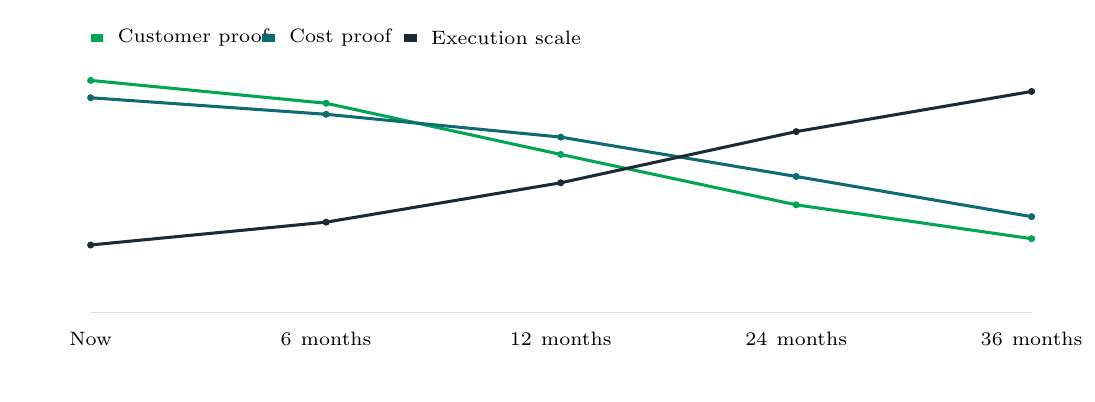
\begin{tikzpicture}[x=1cm,y=1cm]
\path[use as bounding box] (0,0) rectangle (13.20,4.40);
\draw[BOLine] (0.80,0.78) -- (12.75,0.78);
\draw[BOGreen,line width=1.1pt] (0.80,3.73) -- (3.79,3.44) -- (6.77,2.79) -- (9.76,2.15) -- (12.75,1.72);
\fill[BOGreen] (0.80,3.73) circle (.045);
\fill[BOGreen] (3.79,3.44) circle (.045);
\fill[BOGreen] (6.77,2.79) circle (.045);
\fill[BOGreen] (9.76,2.15) circle (.045);
\fill[BOGreen] (12.75,1.72) circle (.045);
\draw[BOBlue,line width=1.1pt] (0.80,3.51) -- (3.79,3.30) -- (6.77,3.01) -- (9.76,2.51) -- (12.75,2.00);
\fill[BOBlue] (0.80,3.51) circle (.045);
\fill[BOBlue] (3.79,3.30) circle (.045);
\fill[BOBlue] (6.77,3.01) circle (.045);
\fill[BOBlue] (9.76,2.51) circle (.045);
\fill[BOBlue] (12.75,2.00) circle (.045);
\draw[BONavy,line width=1.1pt] (0.80,1.64) -- (3.79,1.93) -- (6.77,2.43) -- (9.76,3.08) -- (12.75,3.59);
\fill[BONavy] (0.80,1.64) circle (.045);
\fill[BONavy] (3.79,1.93) circle (.045);
\fill[BONavy] (6.77,2.43) circle (.045);
\fill[BONavy] (9.76,3.08) circle (.045);
\fill[BONavy] (12.75,3.59) circle (.045);
\node[anchor=north,align=center,text width=1.8cm] at (0.80,0.66) {\scriptsize Now};
\node[anchor=north,align=center,text width=1.8cm] at (3.79,0.66) {\scriptsize 6 months};
\node[anchor=north,align=center,text width=1.8cm] at (6.77,0.66) {\scriptsize 12 months};
\node[anchor=north,align=center,text width=1.8cm] at (9.76,0.66) {\scriptsize 24 months};
\node[anchor=north,align=center,text width=1.8cm] at (12.75,0.66) {\scriptsize 36 months};
\fill[BOGreen] (0.80,4.22) rectangle (0.96,4.32);
\node[anchor=west] at (1.02,4.27) {\scriptsize Customer proof};
\fill[BOBlue] (2.98,4.22) rectangle (3.14,4.32);
\node[anchor=west] at (3.20,4.27) {\scriptsize Cost proof};
\fill[BONavy] (4.78,4.22) rectangle (4.94,4.32);
\node[anchor=west] at (5.00,4.27) {\scriptsize Execution scale};
\end{tikzpicture}\par\vspace{2pt}
\vspace{1pt}\noindent\begin{minipage}[t]{0.92\linewidth}
{\footnotesize\color{BOText} The review agenda should shift from proof gathering toward scaling questions only after the earlier uncertainties narrow.}\par
\end{minipage}\par\vspace{1pt}
\vspace{4pt}{\footnotesize\color{BOText} The review agenda should shift from proof gathering toward scaling questions only after the earlier uncertainties narrow.}\par
{\scriptsize\color{BOMuted} BlueOcean uncertainty-resolution model.}\par
\vspace{9pt}\textcolor{BOLine}{\rule{\linewidth}{0.3pt}}\vspace{8pt}
{\textcolor{BOGreen}{\scriptsize\bfseries EXHIBIT 14}}\par\vspace{4pt}
{\sffamily\fontsize{17}{21}\selectfont\color{BONavy} Competitive posture depends on timing, access and reversibility}\par
{\small\color{BOText} Strategic posture map for Nuclear Fusion Commercialization Outlook and Strategic Implications}\par\vspace{6pt}
\noindent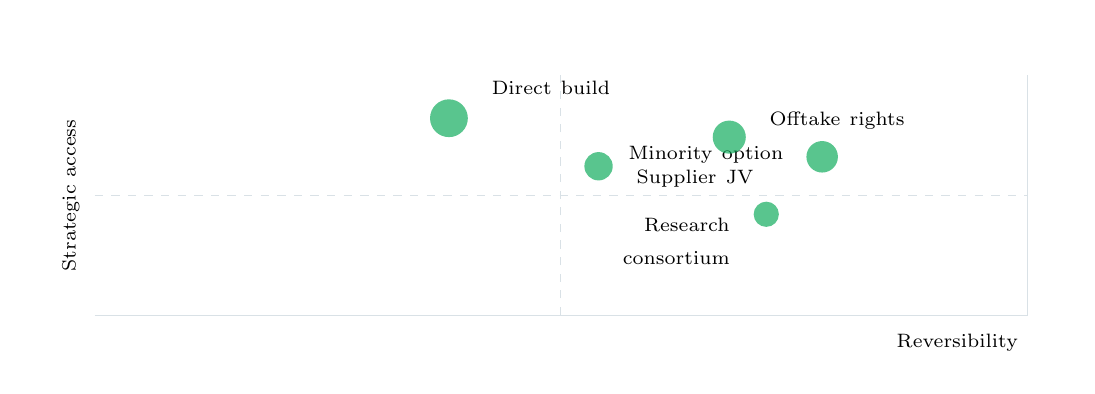
\begin{tikzpicture}[x=1cm,y=1cm]
\path[use as bounding box] (0,0) rectangle (13.20,4.30);
\draw[BOLine] (0.85,0.65) -- (12.70,0.65) -- (12.70,3.70);
\draw[BOLine,dashed] (0.85,2.17) -- (12.70,2.17);
\draw[BOLine,dashed] (6.77,0.65) -- (6.77,3.70);
\fill[BOGreen,opacity=.65] (10.09,2.66) circle (0.20);
\node[anchor=east,align=right,text width=2.10cm] at (9.72,2.69) {\scriptsize Minority option};
\fill[BOGreen,opacity=.65] (8.91,2.91) circle (0.21);
\node[anchor=west,align=left,text width=2.10cm] at (9.30,3.12) {\scriptsize Offtake rights};
\fill[BOGreen,opacity=.65] (7.25,2.54) circle (0.18);
\node[anchor=west,align=left,text width=2.10cm] at (7.61,2.38) {\scriptsize Supplier JV};
\fill[BOGreen,opacity=.65] (5.35,3.15) circle (0.24);
\node[anchor=west,align=left,text width=2.10cm] at (5.77,3.54) {\scriptsize Direct build};
\fill[BOGreen,opacity=.65] (9.38,1.93) circle (0.16);
\node[anchor=east,align=right,text width=2.10cm] at (9.04,1.59) {\scriptsize Research consortium};
\node[anchor=north east] at (12.70,0.53) {\scriptsize Reversibility};
\node[anchor=center,rotate=90] at (0.55,2.17) {\scriptsize Strategic access};
\end{tikzpicture}\par\vspace{2pt}
\vspace{1pt}\noindent\begin{minipage}[t]{0.92\linewidth}
{\footnotesize\color{BOText} Early moves should protect access and learning while avoiding positions that cannot be reversed if evidence weakens.}\par
\end{minipage}\par\vspace{1pt}
\vspace{4pt}{\footnotesize\color{BOText} Early moves should protect access and learning while avoiding positions that cannot be reversed if evidence weakens.}\par
{\scriptsize\color{BOMuted} BlueOcean competitive posture screen.}\par

\clearpage
\label{chap:7}
\noindent\begin{tikzpicture}
\path[use as bounding box] (0,0) rectangle (\linewidth,54mm);
\clip (0,0) rectangle (\linewidth,54mm);
\node[anchor=north west,inner sep=0] at (0,54mm) {
\includegraphics[width=\linewidth]{assets/image-7.png}};
\end{tikzpicture}
\vspace{0pt}
\noindent
\begin{tikzpicture}
\fill[BOGreen] (0,0) rectangle (96mm,1.2pt);
\end{tikzpicture}\par\vspace{8pt}
{\Large\sffamily\bfseries\color{BONavy} Regulation, policy and public acceptance can reset the speed of adoption}\par\vspace{4pt}
{\sffamily\fontsize{15}{20}\selectfont\color{BOGreen} External rules can accelerate the market or change the risk budget and project timeline.}\par\vspace{9pt}
\begin{multicols}{2}
{\small Policy support, permitting rules, standards and public acceptance affect how quickly an opportunity moves from concept to deployment. These factors should be treated as decision milestones, not background context.}\par
{\small Where the regulatory path is unclear, the better move is usually standards engagement, policy tracking and low-risk pilots rather than an early heavy-asset commitment.}\par
{\small The board should track which policy events would change investment timing, such as licensing rules, procurement requirements, subsidy treatment, local approvals or safety standards.}\par
{\small For a CEO, Regulation, policy and public acceptance can reset the speed of adoption matters only if it changes the timing of capital, partner access, customer commitments or risk appetite. The strongest posture is to keep learning close to the business while reserving heavier commitments for proof that can survive investment-committee scrutiny.}\par
{\small For Regulation, policy and public acceptance can reset the speed of adoption, resource allocation should follow the facts that can change the decision: customer demand, cost position, financing availability, regulatory path and delivery capability. If those facts do not improve, increasing exposure mainly creates strategic lock-in rather than higher conviction.}\par
{\small The operating takeaway is that the public record on Regulation, policy and public acceptance can reset the speed of adoption provides a starting point, not a complete underwriting case. The most useful retained signal is: [Source 1: U.S. DOE Fusion Energy Sciences] The Department of Energy has been a leader in fusion energy research since the 1950s and supports groundbreaking advances today. Management should turn that signal into explicit diligence questions rather than a broader claim.}\par
{\small Where Regulation, policy and public acceptance can reset the speed of adoption depends on numbers, the next review should focus on [Source 1: U.S. DOE Fusion Energy Sciences] The Department of Energy has been a leader in fusion energy research since the 1950s and supports groundbreaking advances today.. Those figures determine whether the opportunity belongs in budget planning, option building or continued monitoring.}\par
\end{multicols}
\label{chap:7:end}

\clearpage
\label{chap:8}
\noindent\begin{tikzpicture}
\path[use as bounding box] (0,0) rectangle (\linewidth,54mm);
\clip (0,0) rectangle (\linewidth,54mm);
\node[anchor=north west,inner sep=0] at (0,54mm) {
\includegraphics[width=\linewidth]{assets/image-8.png}};
\end{tikzpicture}
\vspace{0pt}
\noindent
\begin{tikzpicture}
\fill[BOGreen] (0,0) rectangle (96mm,1.2pt);
\end{tikzpicture}\par\vspace{8pt}
{\Large\sffamily\bfseries\color{BONavy} Supply chain, partners and talent will decide who can act before the market is obvious}\par\vspace{4pt}
{\sffamily\fontsize{15}{20}\selectfont\color{BOGreen} Strategic advantage comes from ecosystem position rather than standalone product capability.}\par\vspace{9pt}
\begin{multicols}{2}
{\small In uncertain markets, early advantage often comes from supply access, partner entry, talent pools and customer learning rather than a single technology claim.}\par
{\small A practical reading is that management should identify which capabilities are scarce and can be secured early: critical supply, engineering delivery, channel partners, service network, financing partners and compliance capacity. Low-cost learning rights can be more valuable than waiting for full market clarity.}\par
{\small Partnerships should create observable proof points. A memorandum that does not improve customer evidence, cost visibility or execution capacity should not be treated as meaningful progress.}\par
{\small For a CEO, Supply chain, partners and talent will decide who can act before the market is obvious matters only if it changes the timing of capital, partner access, customer commitments or risk appetite. The strongest posture is to keep learning close to the business while reserving heavier commitments for proof that can survive investment-committee scrutiny.}\par
{\small For Supply chain, partners and talent will decide who can act before the market is obvious, resource allocation should follow the facts that can change the decision: customer demand, cost position, financing availability, regulatory path and delivery capability. If those facts do not improve, increasing exposure mainly creates strategic lock-in rather than higher conviction.}\par
{\small From a board perspective, the public record on Supply chain, partners and talent will decide who can act before the market is obvious provides a starting point, not a complete underwriting case. The most useful retained signal is: [Source 1: U.S. DOE Fusion Energy Sciences] The Department of Energy has been a leader in fusion energy research since the 1950s and supports groundbreaking advances today. Management should turn that signal into explicit diligence questions rather than a broader claim.}\par
{\small Where Supply chain, partners and talent will decide who can act before the market is obvious depends on numbers, the next review should focus on [Source 1: U.S. DOE Fusion Energy Sciences] The Department of Energy has been a leader in fusion energy research since the 1950s and supports groundbreaking advances today.. Those figures determine whether the opportunity belongs in budget planning, option building or continued monitoring.}\par
\end{multicols}
\label{chap:8:end}

\clearpage
{\sffamily\fontsize{20}{25}\selectfont\color{BONavy} About the research}\par\vspace{6pt}
\vspace{2pt}{\color{BOBright}\rule{\linewidth}{1pt}}\vspace{5pt}
{\footnotesize\color{BOMuted} This report has been prepared for strategy discussion and executive decision support. It is not investment, legal, tax, audit or valuation advice. Market estimates, forecasts and scenarios are directional and should be independently validated before they are used for investment, financing, transaction, regulatory or operational decisions. Forward-looking views may change as technology, policy, financing, regulation, competition, supply chains and macro conditions evolve. This report was informed by public research and data from: Osti, Iter, Nationalacademies, Llnl. Detailed references are retained separately rather than reproduced in the client-facing document. Recipients should perform their own diligence and treat this report as one input into a broader decision process.}

\clearpage
\noindent
\begin{tikzpicture}
\fill[BOGreen] (0,0) rectangle (32mm,1.2pt);
\end{tikzpicture}\par\vspace{8pt}
{\sffamily\fontsize{24}{30}\selectfont\color{BONavy} About BlueOcean}\par\vspace{10pt}
\begin{minipage}[t]{0.44\linewidth}
{\sffamily\fontsize{16}{22}\selectfont\color{BOGreen} Research is most useful when it changes a management decision.}\par\vspace{8pt}
{\footnotesize\color{BOText} BlueOcean prepares decision-focused research for executives who need to separate credible evidence from market noise, translate technology shifts into commercial implications and stage commitments around proof.}\par\vspace{7pt}
{\footnotesize\color{BOMuted} This report draws on Osti, Iter, Nationalacademies, Llnl.}\par
\end{minipage}\hfill\begin{minipage}[t]{0.48\linewidth}
\begin{tabularx}{\linewidth}{p{31mm}Y}
{\small\bfseries This report was prepared by the Strategic Energy Research Group, a team}\par{\scriptsize\color{BOGreen} Research synthesis team} & {\footnotesize Responsible for evidence checks, executive synthesis and report QA.} \\[7pt]
\end{tabularx}
\end{minipage}


\clearpage
\thispagestyle{empty}
\begin{tikzpicture}[remember picture,overlay]
\node[anchor=south west,inner sep=0] at (current page.south west) {
\includegraphics[width=\paperwidth,height=\paperheight]{assets/cover-ai.png}};
\fill[black,opacity=.45] (current page.south west) rectangle (current page.north east);
\node[anchor=south east] at ([xshift=-11mm,yshift=10mm]current page.south east) {\sffamily\bfseries\Large\color{white} BlueOcean};
\end{tikzpicture}

\end{document}
